

\section{Implementation}
\label{section:implementation}

We extract aliases for entities from Wikipedia automatically both using API 
and using the actual page content, then apply pattern matching rules for slot 
value extraction. Our contribution is that we perform pattern matching that conforms to each slot 
value along with post-processings to eliminate noisy outputs. 

%\ceg{Instead of this paragraph we talk about what this %section will
%contain. We can discuss the input/output of the system %too.
%}

\subsection{Alias Generation}
\label{section:aliasgeneration}

We use Wikipedia API to get some aliases automatically. This is done by 
retrieving backlink references (redirects of a wiki entity). Unfortunately 
this is not good enough and to enhance recall we need more aliases. To have 
better use of a wiki page we parse HTML DOM of the page, then use regular 
expressions to extract the bold phrases of the first paragraph as alias of the 
actual entity. Based on our observation this is a very accurate heuristic and 
provides us with lots of famous aliases of the entities. To consider other 
typical cases we consider some generic first name last name order swapping 
conventions such as Bill Gates $\rightarrow$ Gates, Bill.  Meanwhile, William Henry
Gates is an alias for Bill Gates in WP as a backlink reference. These kinds of
aliases are also included in matching entities. 

\subsection{Cumulative Citation Recommendation}
\label{sec:ccrimpl}

Our pipeline of processing the corpus consists of a two layer indexing system 
referred to as \textit{Chunk Files Index Generator} and \textit{StreamItems Index Generator}.
Chunk Files Index Generator will generate indexes of the chunk files 
that contain a mention of any of the desired entities. StreamItems Index Generator 
on the other hand will index StreamItems that contain a mention of a given entity 
respectively. This two level indexing will eliminate the need to process each and 
every ChunkFile/StreamItem for every entity. The reason for splitting this task 
into two steps is that not all chunk files contain any mention of the entities and 
we want to get rid of them as soon as possible. Chunk Files Index Generator which 
is written in C++ will discard non-mentioning chunk files and will stop further 
processing a chunk file as soon as it finds a mention there. Each chunk file can 
contain up to thousands of SIs which can be so time consuming if we were to 
process them in our Java base code.Processing StreamItems on the other hand is 
done in Java with ideas in mind for later on extensibility by adding other Java libraries.



\subsection{Streaming Slot Value Extraction}
\label{sec:ssve}
\begin{figure}
\centering
%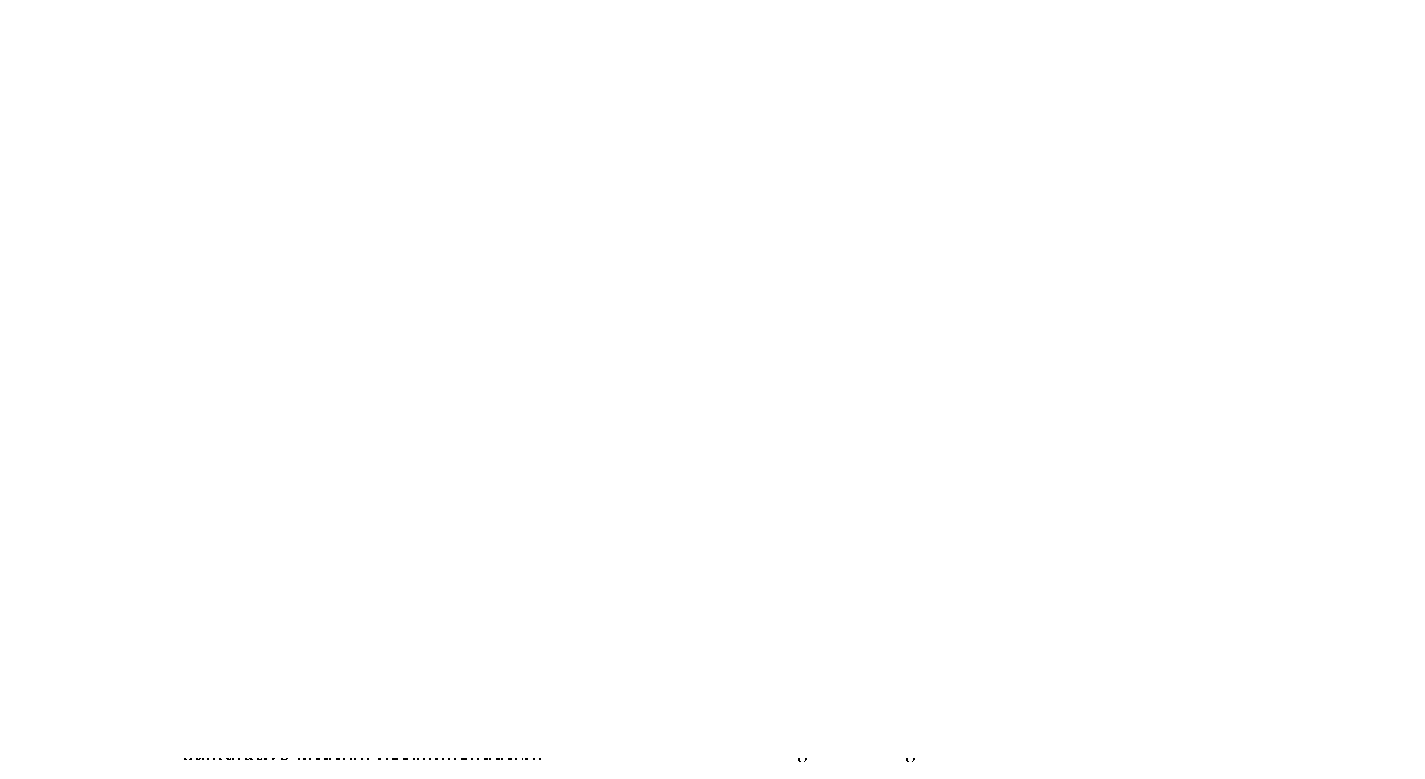
\includegraphics[width=4.5in]{./images/system.eps}
%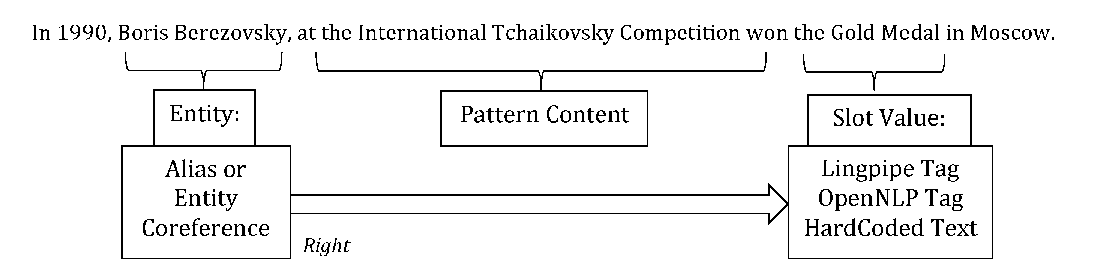
\includegraphics[width=6in]{./images/Pattern.eps}
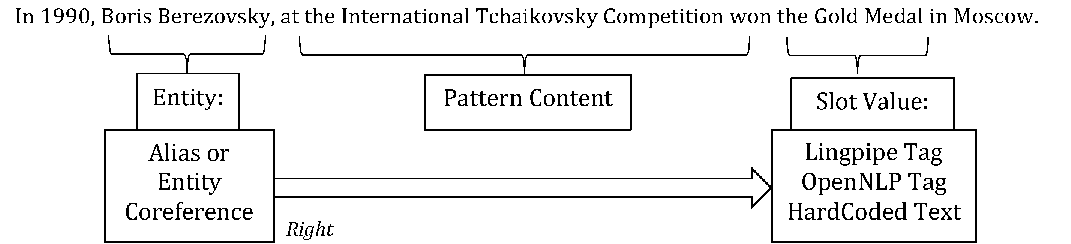
\includegraphics[width=6in]{./images/Pattern-eps-converted-to.pdf}
\vspace*{-.1in} \caption{Pattern Matching with Slot Value on the Right Side of Entity. }\label{fig:pattern}
\vspace*{-.2in}
\end{figure}

In the data set, we are given 4 months of data (October 2011 - February 2012) as training data.
Instead of building a classifier we use pattern matching methods to find
corresponding slot values for entities. 
Pattern matching is simple to manipulate results and implement.
Additionally, we can simply to explain and evaluate results.

The procedure to extract slots with the patterns is to 
first find Streamitems that contain the 
entities by using alias names of the entities. Next, inside these Streamitems, 
fetch the sentences which contain entities by using alias names and the 
coreference information provided by Lingpipe tags. Use these sentences to 
match existing patterns, and when patterns matched, generate SSF results.

\begin{algorithm}
  \textbf{Given a set of Streamitems $\mathcal{S} = \{s_0, \ldots, s_{|\mathcal{S}|}\}$}\\
  \textbf{Set of patterns $P = \{p_0, \ldots, p_{|P|}\}$}\\
  \begin{algorithmic}[1]
    \FOR{$si \in \mathcal{S}$}
    \FOR{$s \in si$}
    \IF{$ check\_one\_of\_the\_patterns$}
    \STATE Emit(sentence, pattern)
  \ENDIF
\ENDFOR
\ENDFOR
\end{algorithmic}
\end{algorithm}


A pattern is defined as a record representing knowledge going to be added to a knowledge base.
A pattern $\mathcal{P}$ is represented as $\mathcal{P} = \langle p_1, p_2, p_3, p_4, p_5 \rangle$.

The first value, $p_1$ represents the type of entity. These entity types are in
the set $\{ \text{\tt FAC}, \text{\tt ORG}, \text{\tt PER} \}$ where \texttt{FAC}
represents a type of facility, \texttt{ORG} represents an organization and \texttt{PER}
represents a person.
The $p_2$ represents a slot name.
A list of slot names is present in Table~\ref{table:slotNameOntology}.
The third element $p_3$ is the pattern content. This is a string found in the sentence.
The extractor looks for this exact string or pattern in a sentence.
The pattern evaluator uses a direction (\texttt{left} or \texttt{right}) found in
$p_4$ to explore sentence.
The final element $p_5$ represent the slot value of a pattern. Thois
%When we match one pattern, we match all the 
%fields except the third field, which is extracted as the final result.
The type of slot value may be the entity 
type tagged by Lingpipe, a noun phrase (\texttt{NP}) tagged by OpenNLP or a hard-coded phrase. 
For these three kinds of patterns, we implement them in different 
ways accordingly. Next we will explain the patterns with more details, a brief
example can be found in Figure~\ref{fig:pattern}. 

\textbf{Slot value type, tagged by Lingpipe:} For slot FounderOf, we have this
pattern: \textless \texttt{PER, FounderOf, ``founder'', right, ORG}\textgreater. PER means 
that the entity we are finding slot values for is a PER entity; FounderOf 
means this is a pattern for FounderOf slot. Founder is the anchor word we are 
trying to match in the sentence text; right means that we are going to the 
right part of the sentence to match the pattern and find the slot value; ORG 
means the slot value should be a ORG entity.

\textbf{Slot value tagged as noun phrase by OpenNLP:} \textless \texttt{PER, AwardsWon, ``awarded'', 
right, NP}\textgreater, NP meaning noun phrase. This pattern can be interpreted 
as that we are looking for a noun phrase after the ``awarded'' since that noun 
phrase could possibly represent an award. Since titles and awards are usually 
not the Lingpipe entities, we use the OpenNLP noun phrase chunker to fetch the 
noun phrases.

\textbf{Slot value of time phrases, hard coded:} \textless \texttt{PER, DateOfDeath, ``died'', right, 
``last night''}\textgreater. In this pattern, ``last night'' means we are looking for 
exactly the phrase ``last night'' to the right of ``died''. This pattern is 
inspired by the intuition that in news articles, people often mention that 
somebody died last night instead of mentioning the accurate date information 
and Lingpipe tends not to tag phrases like ``last night'' as a DATE entity. 

We have found that there are three major classes of accuracy errors:
wrong entities found, wrong tags by the Lingpipe, and finally wrong results matched 
by the patterns. We solve the first problem by using the Wikipedia or twitter 
information of the entities to get better alias names. And we use
post-processing to reduce the second and third types of errors (Section~\ref{section:highAccuracyFilter}).

\subsection{High Accuracy Filter}
\label{section:highAccuracyFilter}

The SSF output of many extractions is noisy. The data contains duplicates and 
incorrect extractions. We can define rules to sanitize the output only using 
the information present in the SSF file. The file is processed in time order, 
in a tuple-at-a-time fashion to minimize the impact on accuracy. We define 
two classes of rules: deduplication rules and inference rules.

The output contains many duplicate entries. As we read the list of extracted 
slots we create rules to define ``duplicate''. Duplicates can be present in a 
window of rows; we use a window size of 2 meaning we only be adjacent rows. 
Two rows are duplicates if they have the same exact extraction, or if the 
rows have the same slot name and a similar slot value or if the extracted 
sentence for a particular slot types come from the same sentence.

 New slots can be deduced from existing slots by defining inference rules. 
 For example, two slots for the task are ``FounderOf'' and ``FoundedBy''. A safe 
 assumption is these slot names are biconditional logical connectives with the 
 entities and slot values. Therefore, we can express a rule ``X FounderOf Y'' 
 equals ``Y FoundedBy X'' where X and Y are single unique entities. Additionally,
 we found that the slot names ``Contact\_Meet\_PlaceTime'' could be inferred as
 ``Contact\_Meet\_Entity'' if the Entity was a FAC and the extracted sentence 
 contained an additional ORG/FAC tag.  
We also remove erronious slots that have extractions that are several pages in 
length or tool small. Errors of extracting long sentences can typically be 
attributed to poor sentence parsing of web documents. We have some valid
``small'' extractions. For example a comma may separate a name and a title
(e.g. ``John, Professor at MIT''). But such extraction rules can be particularly 
noisy, so we check to see if the extracted values have good entity values.


% Note: Talk about how each of the algorithms were created

% Note: Give enough information for our algorithms to be
% reimplemented and verified.

